\documentclass[aspectratio=169,11pt]{beamer}
\usepackage{fontspec,xeCJK}
\setmainfont{texgyreheros-regular.otf}[BoldFont=texgyreheros-bold.otf,ItalicFont=texgyreheros-italic.otf]
\setsansfont{texgyreheros-regular.otf}[BoldFont=texgyreheros-bold.otf,ItalicFont=texgyreheros-italic.otf]
\setCJKmainfont{HaranoAjiGothic-Regular.otf}[BoldFont=HaranoAjiGothic-Bold.otf]
\setCJKsansfont{HaranoAjiGothic-Regular.otf}[BoldFont=HaranoAjiGothic-Bold.otf]
\usepackage{amsmath,amssymb,booktabs,array,tikz}
\usetikzlibrary{arrows.meta,patterns,decorations.markings}
\definecolor{ink}{HTML}{17324D}
\definecolor{accent}{HTML}{157C85}
\definecolor{light}{HTML}{EFF5F6}
\definecolor{muted}{HTML}{536575}
\setbeamercolor{normal text}{fg=ink,bg=white}
\setbeamercolor{frametitle}{fg=ink,bg=white}
\setbeamercolor{structure}{fg=accent}
\setbeamercolor{block title}{fg=white,bg=accent}
\setbeamercolor{block body}{fg=ink,bg=light}
\setbeamerfont{frametitle}{size=\Large,series=\bfseries}
\setbeamersize{text margin left=8mm,text margin right=8mm}
\setbeamertemplate{navigation symbols}{}
\setbeamertemplate{frametitle}{\vspace{2mm}\insertframetitle\par\vspace{1.5mm}{\color{accent}\hrule height .6pt}}
\setbeamertemplate{footline}{\hspace{8mm}\color{muted}\fontsize{6}{7}\selectfont Zenstudy\quad 熱力学\hfill\insertframenumber\hspace{8mm}\vspace{2mm}}
\setlength{\parskip}{3pt}
\newcommand{\tagline}[1]{{\small\color{accent}\textbf{#1}}\par\vspace{1mm}}
\newcommand{\ask}[2]{\par\vspace{2mm}\textcolor{accent}{\textbf{(#1)}}\quad #2\par}
\newcommand{\baseeq}{pV=nRT,\qquad U=\frac32nRT,\qquad Q=\Delta U+W}
\newcommand{\cyclefig}{%
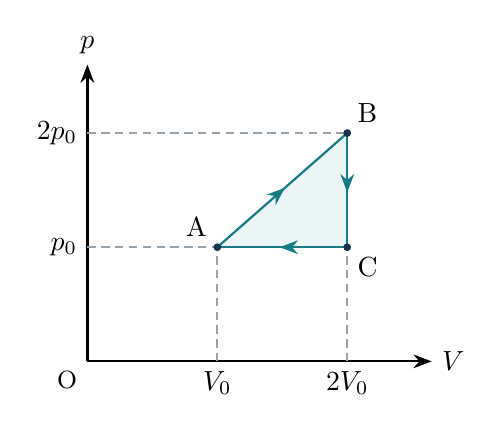
\begin{tikzpicture}[x=1.65cm,y=1.45cm,>=Stealth,line width=.8pt]
\fill[accent!8] (1,1)--(2,2)--(2,1)--cycle;
\draw[->] (0,0)--(2.65,0) node[right]{$V$};
\draw[->] (0,0)--(0,2.6) node[above]{$p$};
\node[below left] at (0,0) {\small O};
\draw[densely dashed,muted!60] (0,1)--(1,1) (0,2)--(2,2) (1,0)--(1,1) (2,0)--(2,1);
\node[left] at (0,1) {$p_0$}; \node[left] at (0,2) {$2p_0$};
\node[below] at (1,0) {$V_0$}; \node[below] at (2,0) {$2V_0$};
\draw[accent,thick,postaction={decorate},decoration={markings,mark=at position .52 with {\arrow{Stealth}}}] (1,1)--(2,2);
\draw[accent,thick,postaction={decorate},decoration={markings,mark=at position .52 with {\arrow{Stealth}}}] (2,2)--(2,1);
\draw[accent,thick,postaction={decorate},decoration={markings,mark=at position .52 with {\arrow{Stealth}}}] (2,1)--(1,1);
\foreach \x/\y in {1/1,2/2,2/1}{\fill[ink] (\x,\y) circle(1.4pt);}
\node[above left] at (1,1) {A}; \node[above right] at (2,2) {B}; \node[below right] at (2,1) {C};
\end{tikzpicture}}
\newcommand{\pistonfig}{%
\begin{tikzpicture}[x=.82cm,y=.82cm,>=Stealth,line width=.8pt]
\fill[accent!8] (.25,.25) rectangle(3.3,2.55);
\fill[pattern=north east lines,pattern color=muted!50] (0,0) rectangle(.25,2.8);
\fill[pattern=north east lines,pattern color=muted!50] (0,2.55) rectangle(4.8,2.8);
\fill[pattern=north east lines,pattern color=muted!50] (0,0) rectangle(4.8,.25);
\draw[thick] (4.8,0)--(0,0)--(0,2.8)--(4.8,2.8);
\draw[thick] (4.8,.25)--(.25,.25)--(.25,2.55)--(4.8,2.55);
\filldraw[fill=muted!25,thick] (3.3,.25) rectangle(3.58,2.55);
\draw[very thick,<-] (3.58,1.4)--(5.4,1.4) node[right]{$F$};
\node at (1.7,1.65) {理想気体};
\node at (1.7,1.05) {$p,\ V,\ T$};
\node[font=\small] at (4.45,2.1) {真空};
\draw[fill=white,line width=1.4pt,accent] (1.05,.08)--(2.1,.08);
\draw[accent,->] (1.55,-.65)--(1.55,.0);
\node[below,font=\small] at (1.55,-.65) {熱窓（開閉式）};
\draw[muted] (3.45,2.58)--(3.45,3.15);
\node[above,font=\small] at (3.45,3.15) {ピストン・断面積 $S$};
\end{tikzpicture}}

\hypersetup{pdftitle={熱力学 基本演習4題 問題 28ポイント版},pdfauthor={Zenstudy 教材制作}}
\begin{document}
\pagehead{第1問　三角形のサイクル／設定}
\cols{
$n\,\mathrm{mol}$ の単原子分子理想気体を、図の順にゆっくり変化させる。
\[
\mathrm{A\to B\to C\to A}
\]
BC は直線で、この過程では全区間で吸熱する。\par
$p_0,V_0>0$ とし、A の温度を $T_0$、気体定数を $R$ とする。
}{\centering\cyclefig}

\newpage
\pagehead{第1問　三角形のサイクル／設問}
\cols{
\ask{1}{B、C の温度を、それぞれ $T_0$ を用いて表せ。}
\ask{2}{各過程の仕事 $W$、内部エネルギーの変化 $\Delta U$、熱量 $Q$ を、$p_0V_0$ を用いて表せ。}
\ask{3}{1周の正味の仕事と、熱効率 $\eta$ を求めよ。}
}{
\labelhead{使ってよい関係式}
\[
U=\frac32nRT,\quad Q=\Delta U+W
\]
$W$ は気体が外部にした仕事で、膨張のとき正。\par
$Q$ は気体が吸収した熱量で、放熱のとき負。\par
熱効率は、正味の仕事を吸収した熱量で割った値。
}

\newpage
\pagehead{第2問　鉛直ピストン／装置}
\cols{
鉛直な断熱円筒に、$n\,\mathrm{mol}$ の単原子分子理想気体を閉じ込める。\par
ピストンの質量は $M$、断面積は $S$ で、摩擦なく上下に動く。\par
上側の大気圧は $p_{\mathrm a}$、重力加速度は $g$ とする。
}{\centering\pistonfig}

\newpage
\pagehead{第2問　鉛直ピストン／初期状態・操作}
\cols{
熱の出入り口は開閉でき、閉じると熱は移動しない。気体は漏れない。\par
初めは追加の外力なしで静止している。圧力・体積・温度を $p_0,V_0,T_0$ とする。
\ask{1}{$p_0$ を $p_{\mathrm a},M,S,g$ で表せ。}
}{
\labelhead{I　A$\to$B}
追加の外力を加えずに加熱し、体積を $2V_0$ にする。\par
\labelhead{II　B$\to$C}
ピストンを固定し、さらに加熱して温度を $4T_0$ にする。\par
操作 I〜III は、ほぼつり合いを保つように十分ゆっくり行う。
}

\newpage
\pagehead{第2問　鉛直ピストン／続き}
\cols{
\labelhead{III　C$\to$D}
熱の出入り口を閉じる。\par
下向きの外力 $F$ をつり合う値に調整し、固定を外す。\par
$F$ を徐々に増やして、体積が $V_0$ になるまで圧縮する。
}{
\ask{2}{B、C の圧力と温度を、$p_0,T_0$ を用いて表せ。}
\ask{3}{操作 I、II のそれぞれで、気体がした仕事 $W$ と吸収した熱量 $Q$ を求めよ。}
\ask{4}{D の温度と、操作 III で気体が外部からされた仕事 $W_{\mathrm{on}}$ を求めよ。}
}

\newpage
\pagehead{第2問　鉛直ピストン／使ってよい関係式}
\cols{
状態方程式と内部エネルギーは、
\[
pV=nRT,\quad U=\frac32nRT.
\]
初期状態について、
\[
p_0V_0=nRT_0.
\]
断熱変化では、
\[
pV^{5/3}=\text{一定}.
\]
}{
熱力学第1法則は、
\[
Q=\Delta U+W.
\]
$W$ は気体が外部にした仕事で、膨張のとき正。\par
$Q$ は気体が吸収した熱量で、放熱のとき負。\par
$W_{\mathrm{on}}$ は、外部から気体にされた仕事の総量とする。
}

\newpage
\pagehead{第3問　状態方程式と内部エネルギー}
\cols{
単原子分子理想気体が、次の状態にある。
\begin{align*}
n&=0.50\,\mathrm{mol},\\
p&=1.0\times10^5\,\mathrm{Pa},\\
V&=1.2\times10^{-2}\,\mathrm{m^3}.
\end{align*}
気体定数は、
\[
R=8.0\,\mathrm{J/(mol\cdot K)}.
\]
}{
\ask{1}{初めの絶対温度 $T$ と内部エネルギー $U$ を求めよ。}
\ask{2}{体積を変えずに加熱し、圧力を $1.5\times10^5\,\mathrm{Pa}$ にした。加熱後の温度 $T'$ と内部エネルギーの変化 $\Delta U$ を求めよ。}
\[
pV=nRT,\quad U=\frac32nRT
\]
を用いてよい。
}

\newpage
\pagehead{第4問　熱気球が浮く条件／設定}
\cols{
熱気球の体積は、
\[
V=1.0\times10^3\,\mathrm{m^3}.
\]
内部の空気を除いた本体・かごなどの質量は、
\[
M=300\,\mathrm{kg}.
\]
外気の温度と密度は、
\[
T_0=300\,\mathrm K,
\]
\[
\rho_0=1.2\,\mathrm{kg/m^3}.
\]
}{\centering\balloonfig}

\newpage
\pagehead{第4問　熱気球が浮く条件／設問}
\cols{
下部が開いているため内外の圧力は等しく、加熱中も体積は一定である。\par
内部の温度は一様で、内外の空気を同じ理想気体とする。
\[
g=10\,\mathrm{m/s^2}.
\]
一定圧力では $\rho T=\text{一定}$。浮力は、押しのけた外気の重さに等しい。
}{
\ask{1}{内部の温度が $400\,\mathrm K$ のとき、空気の密度 $\rho$ を求めよ。}
\ask{2}{このときの浮力と、気球全体に働く上向きの合力を求めよ。}
\ask{3}{静止状態から浮き上がるための、温度 $T$ の条件を求めよ。}
気球の体積以外による浮力と空気抵抗は無視する。
}
\end{document}
